\chapter{Task 3}
Q: Set of states
$\Sigma$: Input alphabet ($\Sigma$ = \{0, 1, \#\})\\
$\Gamma$: Stack alphabet ($\Gamma$ = \{0, 1, $Z_0$\})\\
$\sigma$: Transition function \\
$q_0$: Start state\\
$Z_0$: Initial stack symbol\\
F: Set of accepting states \\
%
$Q = {q_0, q_1, q_2, q_3, q_4, q_5}$ \\
$\Sigma$ = \{0, 1, \#\} \\
$\Gamma$ = \{0, 1, \#, $Z_0$\} \\
$q_0$ = Start state
$Z_0$ = Initial stack symbol \\
$F = {q_5}$ \\
%
The transition function $\sigma$ is defined as follows: \\
%
    $\sigma(q_0, \epsilon, Z_0) = (q_1, Z_0)$ - Move to q1 and push Z0 onto the stack.\\
$\sigma(q_1, 0, Z_0) = (q_1, 0Z_0)$ - Push 0 onto the stack.\\
$\sigma(q_1, 1, Z_0) = (q_1, 1Z_0)$ - Push 1 onto the stack.\\
$\sigma(q_1, \#, Z_0) = (q_2, Z_0)$ - Move to q2 and pop Z0 from the stack.\\
$\sigma(q_2, \epsilon, Z_0) = (q_3, Z_0)$ - Move to q3 and push Z0 onto the stack.\\
$\sigma(q_3, 0, 0) = (q_3, 0)$ - Match 0 on the stack.\\
$\sigma(q_3, 1, 1) = (q_3, 1)$ - Match 1 on the stack.\\
$\sigma(q_3, \epsilon, Z_0) = (q_4, Z_0)$ - Move to q4 and pop Z0 from the stack.\\
$\sigma(q_4, \epsilon, Z_0) = (q_5, Z_0)$ - Move to q5 and pop Z0 from the stack.\\


\begin{figure}[hbt]
  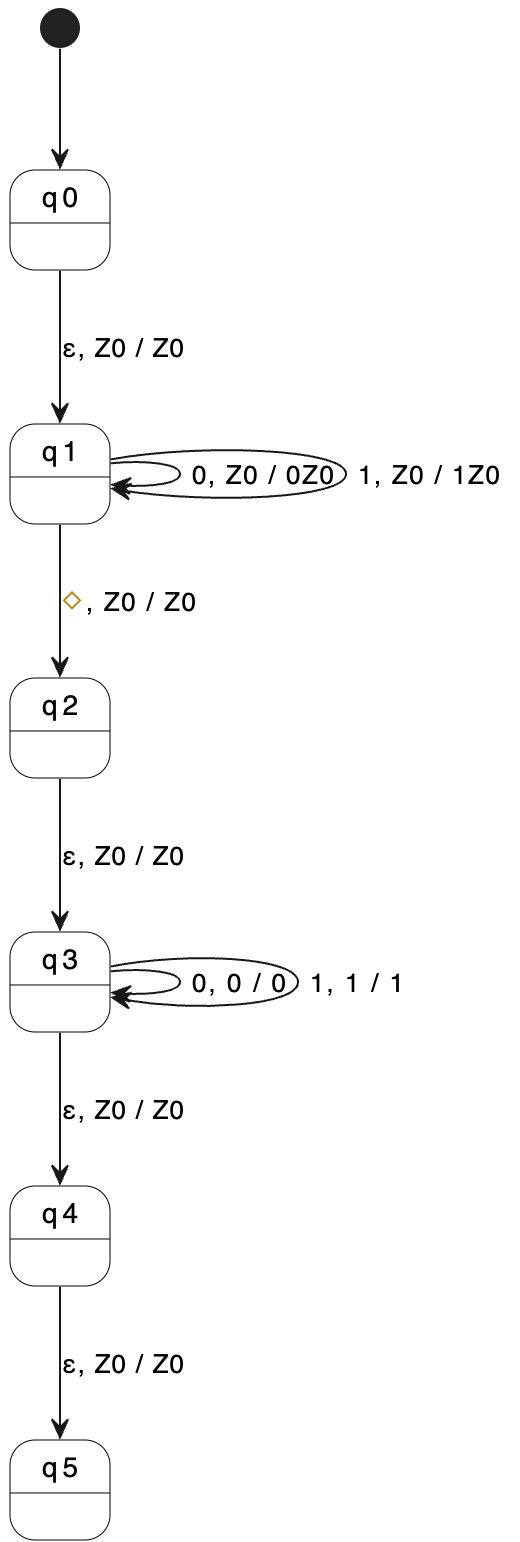
\includegraphics[width=0.5\textwidth]{Immagini/t3}
  \caption{PDA}
\end{figure}
